\documentclass{standalone}
\usepackage{tikz}
\usetikzlibrary{patterns, positioning}

\begin{document}
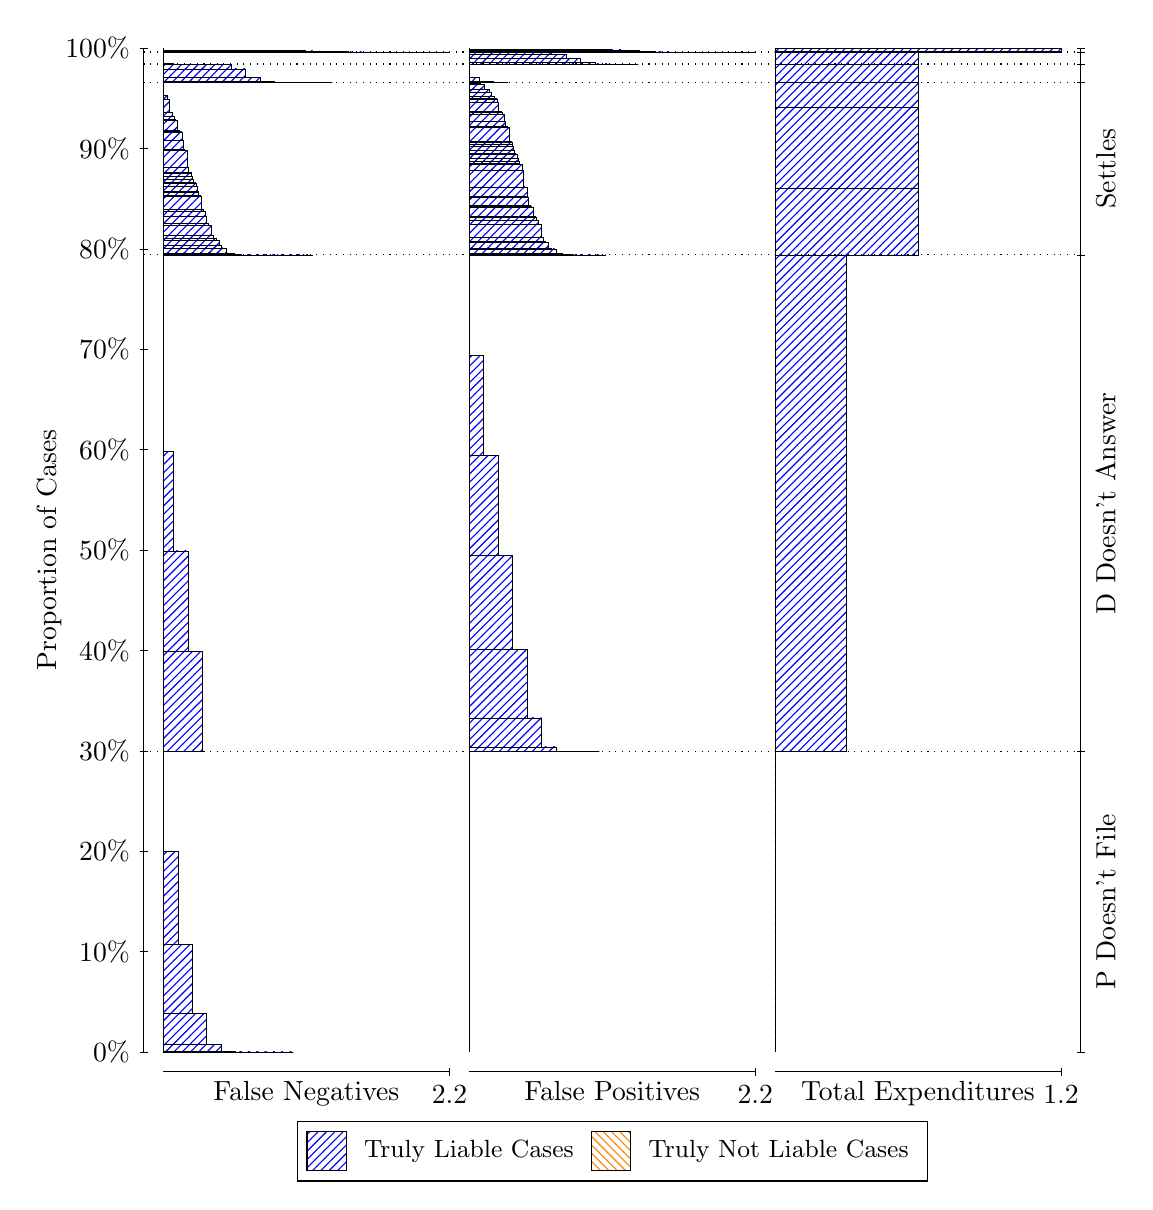
\begin{tikzpicture}
\draw[black, very thin] (1.5,1.75) -- (1.5,14.5);
\node[rotate=90, anchor=center] at (0.3, 8.125) {Proportion of Cases};
\draw[black, very thin] (1.45,1.75) -- (1.55,1.75);
\node[anchor=east] at (1.45, 1.75) {0\%};
\draw[black, very thin] (1.45,3.025) -- (1.55,3.025);
\node[anchor=east] at (1.45, 3.025) {10\%};
\draw[black, very thin] (1.45,4.3) -- (1.55,4.3);
\node[anchor=east] at (1.45, 4.3) {20\%};
\draw[black, very thin] (1.45,5.575) -- (1.55,5.575);
\node[anchor=east] at (1.45, 5.575) {30\%};
\draw[black, very thin] (1.45,6.85) -- (1.55,6.85);
\node[anchor=east] at (1.45, 6.85) {40\%};
\draw[black, very thin] (1.45,8.125) -- (1.55,8.125);
\node[anchor=east] at (1.45, 8.125) {50\%};
\draw[black, very thin] (1.45,9.4) -- (1.55,9.4);
\node[anchor=east] at (1.45, 9.4) {60\%};
\draw[black, very thin] (1.45,10.675) -- (1.55,10.675);
\node[anchor=east] at (1.45, 10.675) {70\%};
\draw[black, very thin] (1.45,11.95) -- (1.55,11.95);
\node[anchor=east] at (1.45, 11.95) {80\%};
\draw[black, very thin] (1.45,13.225) -- (1.55,13.225);
\node[anchor=east] at (1.45, 13.225) {90\%};
\draw[black, very thin] (1.45,14.5) -- (1.55,14.5);
\node[anchor=east] at (1.45, 14.5) {100\%};

\draw[black, very thin] (13.4,1.75) -- (13.4,14.5);
\draw[black, very thin] (13.35,1.75) -- (13.45,1.75);
\node[anchor=west] at (13.35, 1.75) {};
\draw[black, very thin] (13.35,5.563) -- (13.45,5.563);
\node[anchor=west] at (13.35, 5.563) {};
\draw[black, very thin] (13.35,11.874) -- (13.45,11.874);
\node[anchor=west] at (13.35, 11.874) {};
\draw[black, very thin] (13.35,14.064) -- (13.45,14.064);
\node[anchor=west] at (13.35, 14.064) {};
\draw[black, very thin] (13.35,14.297) -- (13.45,14.297);
\node[anchor=west] at (13.35, 14.297) {};
\draw[black, very thin] (13.35,14.449) -- (13.45,14.449);
\node[anchor=west] at (13.35, 14.449) {};
\draw[black, very thin] (13.35,14.5) -- (13.45,14.5);
\node[anchor=west] at (13.35, 14.5) {};

\draw[black, very thin, pattern color=blue, pattern=north east lines] (1.75,1.75) rectangle (3.4015,1.75);
\draw[black, very thin, pattern color=blue, pattern=north east lines] (1.75,1.75) rectangle (3.218,1.75);
\draw[black, very thin, pattern color=blue, pattern=north east lines] (1.75,1.75) rectangle (3.0345,1.75);
\draw[black, very thin, pattern color=blue, pattern=north east lines] (1.75,1.75) rectangle (2.851,1.7503);
\draw[black, very thin, pattern color=blue, pattern=north east lines] (1.75,1.7503) rectangle (2.6675,1.7582);
\draw[black, very thin, pattern color=blue, pattern=north east lines] (1.75,1.7582) rectangle (2.484,1.8434);
\draw[black, very thin, pattern color=blue, pattern=north east lines] (1.75,1.8434) rectangle (2.3005,2.2366);
\draw[black, very thin, pattern color=blue, pattern=north east lines] (1.75,2.2366) rectangle (2.117,3.1157);
\draw[black, very thin, pattern color=blue, pattern=north east lines] (1.75,3.1157) rectangle (1.9335,4.2995);
\draw[black, very thin, pattern color=orange, pattern=north west lines] (1.75,4.2995) rectangle (1.75,4.2995);
\draw[black, very thin, pattern color=blue, pattern=north east lines] (1.75,4.2995) rectangle (1.75,5.563);
\draw[black, very thin, pattern color=blue, pattern=north east lines] (1.75,5.563) rectangle (2.2455,6.838);
\draw[black, very thin, pattern color=blue, pattern=north east lines] (1.75,6.838) rectangle (2.062,8.1127);
\draw[black, very thin, pattern color=blue, pattern=north east lines] (1.75,8.1127) rectangle (1.8785,9.3798);
\draw[black, very thin, pattern color=orange, pattern=north west lines] (1.75,9.3798) rectangle (1.75,9.3798);
\draw[black, very thin, pattern color=blue, pattern=north east lines] (1.75,9.3798) rectangle (1.75,11.874);
\draw[black, very thin, pattern color=blue, pattern=north east lines] (1.75,11.874) rectangle (3.6492,11.874);
\draw[black, very thin, pattern color=blue, pattern=north east lines] (1.75,11.874) rectangle (3.5667,11.874);
\draw[black, very thin, pattern color=blue, pattern=north east lines] (1.75,11.874) rectangle (3.4841,11.874);
\draw[black, very thin, pattern color=blue, pattern=north east lines] (1.75,11.874) rectangle (3.4657,11.874);
\draw[black, very thin, pattern color=blue, pattern=north east lines] (1.75,11.874) rectangle (3.4015,11.874);
\draw[black, very thin, pattern color=blue, pattern=north east lines] (1.75,11.874) rectangle (3.3832,11.874);
\draw[black, very thin, pattern color=blue, pattern=north east lines] (1.75,11.874) rectangle (3.3189,11.874);
\draw[black, very thin, pattern color=blue, pattern=north east lines] (1.75,11.874) rectangle (3.3006,11.874);
\draw[black, very thin, pattern color=blue, pattern=north east lines] (1.75,11.874) rectangle (3.2822,11.874);
\draw[black, very thin, pattern color=blue, pattern=north east lines] (1.75,11.874) rectangle (3.2364,11.874);
\draw[black, very thin, pattern color=blue, pattern=north east lines] (1.75,11.874) rectangle (3.218,11.874);
\draw[black, very thin, pattern color=blue, pattern=north east lines] (1.75,11.874) rectangle (3.1997,11.874);
\draw[black, very thin, pattern color=blue, pattern=north east lines] (1.75,11.874) rectangle (3.1538,11.874);
\draw[black, very thin, pattern color=blue, pattern=north east lines] (1.75,11.874) rectangle (3.1354,11.874);
\draw[black, very thin, pattern color=blue, pattern=north east lines] (1.75,11.874) rectangle (3.1171,11.874);
\draw[black, very thin, pattern color=blue, pattern=north east lines] (1.75,11.874) rectangle (3.0987,11.874);
\draw[black, very thin, pattern color=blue, pattern=north east lines] (1.75,11.874) rectangle (3.0712,11.874);
\draw[black, very thin, pattern color=blue, pattern=north east lines] (1.75,11.874) rectangle (3.0529,11.874);
\draw[black, very thin, pattern color=blue, pattern=north east lines] (1.75,11.874) rectangle (3.0345,11.874);
\draw[black, very thin, pattern color=blue, pattern=north east lines] (1.75,11.874) rectangle (3.0162,11.874);
\draw[black, very thin, pattern color=blue, pattern=north east lines] (1.75,11.874) rectangle (2.9886,11.874);
\draw[black, very thin, pattern color=blue, pattern=north east lines] (1.75,11.874) rectangle (2.9703,11.874);
\draw[black, very thin, pattern color=blue, pattern=north east lines] (1.75,11.874) rectangle (2.9519,11.874);
\draw[black, very thin, pattern color=blue, pattern=north east lines] (1.75,11.874) rectangle (2.9336,11.874);
\draw[black, very thin, pattern color=blue, pattern=north east lines] (1.75,11.874) rectangle (2.9152,11.874);
\draw[black, very thin, pattern color=blue, pattern=north east lines] (1.75,11.874) rectangle (2.9061,11.874);
\draw[black, very thin, pattern color=blue, pattern=north east lines] (1.75,11.874) rectangle (2.8877,11.874);
\draw[black, very thin, pattern color=blue, pattern=north east lines] (1.75,11.874) rectangle (2.8694,11.874);
\draw[black, very thin, pattern color=blue, pattern=north east lines] (1.75,11.874) rectangle (2.851,11.874);
\draw[black, very thin, pattern color=blue, pattern=north east lines] (1.75,11.874) rectangle (2.8327,11.874);
\draw[black, very thin, pattern color=blue, pattern=north east lines] (1.75,11.874) rectangle (2.8235,11.874);
\draw[black, very thin, pattern color=blue, pattern=north east lines] (1.75,11.874) rectangle (2.8051,11.874);
\draw[black, very thin, pattern color=blue, pattern=north east lines] (1.75,11.874) rectangle (2.7868,11.874);
\draw[black, very thin, pattern color=blue, pattern=north east lines] (1.75,11.874) rectangle (2.7684,11.874);
\draw[black, very thin, pattern color=blue, pattern=north east lines] (1.75,11.874) rectangle (2.7501,11.874);
\draw[black, very thin, pattern color=blue, pattern=north east lines] (1.75,11.874) rectangle (2.7409,11.874);
\draw[black, very thin, pattern color=blue, pattern=north east lines] (1.75,11.874) rectangle (2.7317,11.881);
\draw[black, very thin, pattern color=blue, pattern=north east lines] (1.75,11.881) rectangle (2.7226,11.881);
\draw[black, very thin, pattern color=blue, pattern=north east lines] (1.75,11.881) rectangle (2.7042,11.881);
\draw[black, very thin, pattern color=blue, pattern=north east lines] (1.75,11.881) rectangle (2.6859,11.881);
\draw[black, very thin, pattern color=blue, pattern=north east lines] (1.75,11.881) rectangle (2.6675,11.883);
\draw[black, very thin, pattern color=blue, pattern=north east lines] (1.75,11.883) rectangle (2.6583,11.883);
\draw[black, very thin, pattern color=blue, pattern=north east lines] (1.75,11.883) rectangle (2.6492,11.892);
\draw[black, very thin, pattern color=blue, pattern=north east lines] (1.75,11.892) rectangle (2.64,11.892);
\draw[black, very thin, pattern color=blue, pattern=north east lines] (1.75,11.892) rectangle (2.6216,11.892);
\draw[black, very thin, pattern color=blue, pattern=north east lines] (1.75,11.892) rectangle (2.6033,11.892);
\draw[black, very thin, pattern color=blue, pattern=north east lines] (1.75,11.892) rectangle (2.5849,11.893);
\draw[black, very thin, pattern color=blue, pattern=north east lines] (1.75,11.893) rectangle (2.5666,11.899);
\draw[black, very thin, pattern color=blue, pattern=north east lines] (1.75,11.899) rectangle (2.5574,11.899);
\draw[black, very thin, pattern color=blue, pattern=north east lines] (1.75,11.899) rectangle (2.5482,11.958);
\draw[black, very thin, pattern color=blue, pattern=north east lines] (1.75,11.958) rectangle (2.5391,11.958);
\draw[black, very thin, pattern color=blue, pattern=north east lines] (1.75,11.958) rectangle (2.5207,11.958);
\draw[black, very thin, pattern color=blue, pattern=north east lines] (1.75,11.958) rectangle (2.5024,11.961);
\draw[black, very thin, pattern color=blue, pattern=north east lines] (1.75,11.961) rectangle (2.484,11.998);
\draw[black, very thin, pattern color=blue, pattern=north east lines] (1.75,11.998) rectangle (2.4748,11.998);
\draw[black, very thin, pattern color=blue, pattern=north east lines] (1.75,11.998) rectangle (2.4657,12.054);
\draw[black, very thin, pattern color=blue, pattern=north east lines] (1.75,12.054) rectangle (2.4565,12.054);
\draw[black, very thin, pattern color=blue, pattern=north east lines] (1.75,12.054) rectangle (2.4381,12.055);
\draw[black, very thin, pattern color=blue, pattern=north east lines] (1.75,12.055) rectangle (2.4198,12.08);
\draw[black, very thin, pattern color=blue, pattern=north east lines] (1.75,12.08) rectangle (2.4014,12.085);
\draw[black, very thin, pattern color=blue, pattern=north east lines] (1.75,12.085) rectangle (2.3831,12.122);
\draw[black, very thin, pattern color=blue, pattern=north east lines] (1.75,12.122) rectangle (2.3739,12.123);
\draw[black, very thin, pattern color=blue, pattern=north east lines] (1.75,12.123) rectangle (2.3647,12.243);
\draw[black, very thin, pattern color=blue, pattern=north east lines] (1.75,12.243) rectangle (2.3556,12.246);
\draw[black, very thin, pattern color=blue, pattern=north east lines] (1.75,12.246) rectangle (2.3372,12.25);
\draw[black, very thin, pattern color=blue, pattern=north east lines] (1.75,12.25) rectangle (2.3189,12.275);
\draw[black, very thin, pattern color=blue, pattern=north east lines] (1.75,12.275) rectangle (2.3005,12.367);
\draw[black, very thin, pattern color=blue, pattern=north east lines] (1.75,12.367) rectangle (2.2913,12.369);
\draw[black, very thin, pattern color=blue, pattern=north east lines] (1.75,12.369) rectangle (2.2822,12.426);
\draw[black, very thin, pattern color=blue, pattern=north east lines] (1.75,12.426) rectangle (2.273,12.426);
\draw[black, very thin, pattern color=blue, pattern=north east lines] (1.75,12.426) rectangle (2.2546,12.448);
\draw[black, very thin, pattern color=blue, pattern=north east lines] (1.75,12.448) rectangle (2.2363,12.62);
\draw[black, very thin, pattern color=blue, pattern=north east lines] (1.75,12.62) rectangle (2.2179,12.629);
\draw[black, very thin, pattern color=blue, pattern=north east lines] (1.75,12.629) rectangle (2.1996,12.666);
\draw[black, very thin, pattern color=blue, pattern=north east lines] (1.75,12.666) rectangle (2.1904,12.681);
\draw[black, very thin, pattern color=blue, pattern=north east lines] (1.75,12.681) rectangle (2.1812,12.741);
\draw[black, very thin, pattern color=blue, pattern=north east lines] (1.75,12.741) rectangle (2.1721,12.777);
\draw[black, very thin, pattern color=blue, pattern=north east lines] (1.75,12.777) rectangle (2.1537,12.792);
\draw[black, very thin, pattern color=blue, pattern=north east lines] (1.75,12.792) rectangle (2.1354,12.833);
\draw[black, very thin, pattern color=blue, pattern=north east lines] (1.75,12.833) rectangle (2.117,12.87);
\draw[black, very thin, pattern color=blue, pattern=north east lines] (1.75,12.87) rectangle (2.1078,12.906);
\draw[black, very thin, pattern color=blue, pattern=north east lines] (1.75,12.906) rectangle (2.0987,12.916);
\draw[black, very thin, pattern color=blue, pattern=north east lines] (1.75,12.916) rectangle (2.0895,12.92);
\draw[black, very thin, pattern color=blue, pattern=north east lines] (1.75,12.92) rectangle (2.0711,12.987);
\draw[black, very thin, pattern color=blue, pattern=north east lines] (1.75,12.987) rectangle (2.0528,13.201);
\draw[black, very thin, pattern color=blue, pattern=north east lines] (1.75,13.201) rectangle (2.0344,13.203);
\draw[black, very thin, pattern color=blue, pattern=north east lines] (1.75,13.203) rectangle (2.0161,13.21);
\draw[black, very thin, pattern color=blue, pattern=north east lines] (1.75,13.21) rectangle (2.0069,13.324);
\draw[black, very thin, pattern color=blue, pattern=north east lines] (1.75,13.324) rectangle (1.9977,13.334);
\draw[black, very thin, pattern color=blue, pattern=north east lines] (1.75,13.334) rectangle (1.9886,13.436);
\draw[black, very thin, pattern color=blue, pattern=north east lines] (1.75,13.436) rectangle (1.9702,13.446);
\draw[black, very thin, pattern color=blue, pattern=north east lines] (1.75,13.446) rectangle (1.9519,13.459);
\draw[black, very thin, pattern color=blue, pattern=north east lines] (1.75,13.459) rectangle (1.9335,13.461);
\draw[black, very thin, pattern color=blue, pattern=north east lines] (1.75,13.461) rectangle (1.9243,13.579);
\draw[black, very thin, pattern color=blue, pattern=north east lines] (1.75,13.579) rectangle (1.9152,13.579);
\draw[black, very thin, pattern color=blue, pattern=north east lines] (1.75,13.579) rectangle (1.906,13.591);
\draw[black, very thin, pattern color=blue, pattern=north east lines] (1.75,13.591) rectangle (1.8876,13.628);
\draw[black, very thin, pattern color=blue, pattern=north east lines] (1.75,13.628) rectangle (1.8693,13.68);
\draw[black, very thin, pattern color=blue, pattern=north east lines] (1.75,13.68) rectangle (1.8509,13.68);
\draw[black, very thin, pattern color=blue, pattern=north east lines] (1.75,13.68) rectangle (1.8326,13.68);
\draw[black, very thin, pattern color=blue, pattern=north east lines] (1.75,13.68) rectangle (1.8234,13.844);
\draw[black, very thin, pattern color=blue, pattern=north east lines] (1.75,13.844) rectangle (1.8051,13.897);
\draw[black, very thin, pattern color=blue, pattern=north east lines] (1.75,13.897) rectangle (1.7867,13.898);
\draw[black, very thin, pattern color=blue, pattern=north east lines] (1.75,13.898) rectangle (1.7684,13.899);
\draw[black, very thin, pattern color=orange, pattern=north west lines] (1.75,13.899) rectangle (1.75,13.899);
\draw[black, very thin, pattern color=blue, pattern=north east lines] (1.75,13.899) rectangle (1.75,14.064);
\draw[black, very thin, pattern color=blue, pattern=north east lines] (1.75,14.064) rectangle (3.897,14.064);
\draw[black, very thin, pattern color=blue, pattern=north east lines] (1.75,14.064) rectangle (3.7135,14.064);
\draw[black, very thin, pattern color=blue, pattern=north east lines] (1.75,14.064) rectangle (3.53,14.064);
\draw[black, very thin, pattern color=blue, pattern=north east lines] (1.75,14.064) rectangle (3.3465,14.064);
\draw[black, very thin, pattern color=blue, pattern=north east lines] (1.75,14.064) rectangle (3.163,14.072);
\draw[black, very thin, pattern color=blue, pattern=north east lines] (1.75,14.072) rectangle (2.9795,14.127);
\draw[black, very thin, pattern color=blue, pattern=north east lines] (1.75,14.127) rectangle (2.796,14.235);
\draw[black, very thin, pattern color=blue, pattern=north east lines] (1.75,14.235) rectangle (2.6125,14.289);
\draw[black, very thin, pattern color=blue, pattern=north east lines] (1.75,14.289) rectangle (2.429,14.296);
\draw[black, very thin, pattern color=blue, pattern=north east lines] (1.75,14.296) rectangle (2.2455,14.297);
\draw[black, very thin, pattern color=orange, pattern=north west lines] (1.75,14.297) rectangle (1.75,14.297);
\draw[black, very thin, pattern color=blue, pattern=north east lines] (1.75,14.297) rectangle (2.2455,14.297);
\draw[black, very thin, pattern color=blue, pattern=north east lines] (1.75,14.297) rectangle (2.062,14.297);
\draw[black, very thin, pattern color=blue, pattern=north east lines] (1.75,14.297) rectangle (1.8785,14.302);
\draw[black, very thin, pattern color=orange, pattern=north west lines] (1.75,14.302) rectangle (1.75,14.302);
\draw[black, very thin, pattern color=blue, pattern=north east lines] (1.75,14.302) rectangle (1.75,14.449);
\draw[black, very thin, pattern color=blue, pattern=north east lines] (1.75,14.449) rectangle (5.3833,14.449);
\draw[black, very thin, pattern color=blue, pattern=north east lines] (1.75,14.449) rectangle (5.1998,14.449);
\draw[black, very thin, pattern color=blue, pattern=north east lines] (1.75,14.449) rectangle (5.0163,14.449);
\draw[black, very thin, pattern color=blue, pattern=north east lines] (1.75,14.449) rectangle (5.0163,14.449);
\draw[black, very thin, pattern color=blue, pattern=north east lines] (1.75,14.449) rectangle (4.8328,14.449);
\draw[black, very thin, pattern color=blue, pattern=north east lines] (1.75,14.449) rectangle (4.6493,14.449);
\draw[black, very thin, pattern color=blue, pattern=north east lines] (1.75,14.449) rectangle (4.4658,14.449);
\draw[black, very thin, pattern color=blue, pattern=north east lines] (1.75,14.449) rectangle (4.2823,14.451);
\draw[black, very thin, pattern color=blue, pattern=north east lines] (1.75,14.451) rectangle (4.0988,14.451);
\draw[black, very thin, pattern color=blue, pattern=north east lines] (1.75,14.451) rectangle (4.0988,14.455);
\draw[black, very thin, pattern color=blue, pattern=north east lines] (1.75,14.455) rectangle (3.9153,14.461);
\draw[black, very thin, pattern color=blue, pattern=north east lines] (1.75,14.461) rectangle (3.9153,14.461);
\draw[black, very thin, pattern color=blue, pattern=north east lines] (1.75,14.461) rectangle (3.7318,14.465);
\draw[black, very thin, pattern color=blue, pattern=north east lines] (1.75,14.465) rectangle (3.5483,14.465);
\draw[black, very thin, pattern color=blue, pattern=north east lines] (1.75,14.465) rectangle (3.5483,14.466);
\draw[black, very thin, pattern color=blue, pattern=north east lines] (1.75,14.466) rectangle (3.3648,14.466);
\draw[black, very thin, pattern color=blue, pattern=north east lines] (1.75,14.466) rectangle (3.3648,14.466);
\draw[black, very thin, pattern color=blue, pattern=north east lines] (1.75,14.466) rectangle (3.3648,14.466);
\draw[black, very thin, pattern color=blue, pattern=north east lines] (1.75,14.466) rectangle (3.1813,14.466);
\draw[black, very thin, pattern color=blue, pattern=north east lines] (1.75,14.466) rectangle (3.1813,14.466);
\draw[black, very thin, pattern color=blue, pattern=north east lines] (1.75,14.466) rectangle (3.0345,14.466);
\draw[black, very thin, pattern color=blue, pattern=north east lines] (1.75,14.466) rectangle (2.9978,14.466);
\draw[black, very thin, pattern color=blue, pattern=north east lines] (1.75,14.466) rectangle (2.851,14.466);
\draw[black, very thin, pattern color=blue, pattern=north east lines] (1.75,14.466) rectangle (2.851,14.466);
\draw[black, very thin, pattern color=blue, pattern=north east lines] (1.75,14.466) rectangle (2.8143,14.466);
\draw[black, very thin, pattern color=blue, pattern=north east lines] (1.75,14.466) rectangle (2.6675,14.466);
\draw[black, very thin, pattern color=blue, pattern=north east lines] (1.75,14.466) rectangle (2.6308,14.466);
\draw[black, very thin, pattern color=blue, pattern=north east lines] (1.75,14.466) rectangle (2.484,14.466);
\draw[black, very thin, pattern color=blue, pattern=north east lines] (1.75,14.466) rectangle (2.484,14.466);
\draw[black, very thin, pattern color=blue, pattern=north east lines] (1.75,14.466) rectangle (2.3005,14.466);
\draw[black, very thin, pattern color=blue, pattern=north east lines] (1.75,14.466) rectangle (2.3005,14.466);
\draw[black, very thin, pattern color=blue, pattern=north east lines] (1.75,14.466) rectangle (2.3005,14.466);
\draw[black, very thin, pattern color=blue, pattern=north east lines] (1.75,14.466) rectangle (2.117,14.466);
\draw[black, very thin, pattern color=blue, pattern=north east lines] (1.75,14.466) rectangle (2.117,14.467);
\draw[black, very thin, pattern color=blue, pattern=north east lines] (1.75,14.467) rectangle (1.9335,14.468);
\draw[black, very thin, pattern color=blue, pattern=north east lines] (1.75,14.468) rectangle (1.9335,14.472);
\draw[black, very thin, pattern color=blue, pattern=north east lines] (1.75,14.472) rectangle (1.9335,14.472);
\draw[black, very thin, pattern color=orange, pattern=north west lines] (1.75,14.472) rectangle (1.75,14.472);
\draw[black, very thin, pattern color=blue, pattern=north east lines] (1.75,14.472) rectangle (1.75,14.5);
\draw[black, very thin, pattern color=orange, pattern=north west lines] (5.6333,1.75) rectangle (5.6333,1.75);
\draw[black, very thin, pattern color=blue, pattern=north east lines] (5.6333,1.75) rectangle (5.6333,5.563);
\draw[black, very thin, pattern color=orange, pattern=north west lines] (5.6333,5.563) rectangle (7.2848,5.563);
\draw[black, very thin, pattern color=blue, pattern=north east lines] (5.6333,5.563) rectangle (7.2848,5.563);
\draw[black, very thin, pattern color=blue, pattern=north east lines] (5.6333,5.563) rectangle (7.1013,5.563);
\draw[black, very thin, pattern color=blue, pattern=north east lines] (5.6333,5.563) rectangle (6.9178,5.5655);
\draw[black, very thin, pattern color=blue, pattern=north east lines] (5.6333,5.5655) rectangle (6.7343,5.6244);
\draw[black, very thin, pattern color=blue, pattern=north east lines] (5.6333,5.6244) rectangle (6.5508,5.9915);
\draw[black, very thin, pattern color=blue, pattern=north east lines] (5.6333,5.9915) rectangle (6.3673,6.8677);
\draw[black, very thin, pattern color=blue, pattern=north east lines] (5.6333,6.8677) rectangle (6.1838,8.0572);
\draw[black, very thin, pattern color=blue, pattern=north east lines] (5.6333,8.0572) rectangle (6.0003,9.3242);
\draw[black, very thin, pattern color=blue, pattern=north east lines] (5.6333,9.3242) rectangle (5.8168,10.599);
\draw[black, very thin, pattern color=blue, pattern=north east lines] (5.6333,10.599) rectangle (5.6333,11.874);
\draw[black, very thin, pattern color=orange, pattern=north west lines] (5.6333,11.874) rectangle (7.3674,11.874);
\draw[black, very thin, pattern color=blue, pattern=north east lines] (5.6333,11.874) rectangle (7.3674,11.874);
\draw[black, very thin, pattern color=orange, pattern=north west lines] (5.6333,11.874) rectangle (7.2848,11.874);
\draw[black, very thin, pattern color=blue, pattern=north east lines] (5.6333,11.874) rectangle (7.2848,11.874);
\draw[black, very thin, pattern color=orange, pattern=north west lines] (5.6333,11.874) rectangle (7.2023,11.874);
\draw[black, very thin, pattern color=blue, pattern=north east lines] (5.6333,11.874) rectangle (7.2023,11.874);
\draw[black, very thin, pattern color=blue, pattern=north east lines] (5.6333,11.874) rectangle (7.1839,11.874);
\draw[black, very thin, pattern color=orange, pattern=north west lines] (5.6333,11.874) rectangle (7.1197,11.874);
\draw[black, very thin, pattern color=blue, pattern=north east lines] (5.6333,11.874) rectangle (7.1197,11.874);
\draw[black, very thin, pattern color=blue, pattern=north east lines] (5.6333,11.874) rectangle (7.1013,11.874);
\draw[black, very thin, pattern color=orange, pattern=north west lines] (5.6333,11.874) rectangle (7.0371,11.874);
\draw[black, very thin, pattern color=blue, pattern=north east lines] (5.6333,11.874) rectangle (7.0371,11.874);
\draw[black, very thin, pattern color=blue, pattern=north east lines] (5.6333,11.874) rectangle (7.0188,11.874);
\draw[black, very thin, pattern color=blue, pattern=north east lines] (5.6333,11.874) rectangle (7.0004,11.874);
\draw[black, very thin, pattern color=orange, pattern=north west lines] (5.6333,11.874) rectangle (6.9545,11.874);
\draw[black, very thin, pattern color=blue, pattern=north east lines] (5.6333,11.874) rectangle (6.9545,11.874);
\draw[black, very thin, pattern color=blue, pattern=north east lines] (5.6333,11.874) rectangle (6.9362,11.875);
\draw[black, very thin, pattern color=blue, pattern=north east lines] (5.6333,11.875) rectangle (6.9178,11.878);
\draw[black, very thin, pattern color=orange, pattern=north west lines] (5.6333,11.878) rectangle (6.872,11.878);
\draw[black, very thin, pattern color=blue, pattern=north east lines] (5.6333,11.878) rectangle (6.872,11.878);
\draw[black, very thin, pattern color=blue, pattern=north east lines] (5.6333,11.878) rectangle (6.8536,11.878);
\draw[black, very thin, pattern color=blue, pattern=north east lines] (5.6333,11.878) rectangle (6.8353,11.879);
\draw[black, very thin, pattern color=blue, pattern=north east lines] (5.6333,11.879) rectangle (6.8169,11.891);
\draw[black, very thin, pattern color=orange, pattern=north west lines] (5.6333,11.891) rectangle (6.7894,11.891);
\draw[black, very thin, pattern color=blue, pattern=north east lines] (5.6333,11.891) rectangle (6.7894,11.891);
\draw[black, very thin, pattern color=blue, pattern=north east lines] (5.6333,11.891) rectangle (6.771,11.891);
\draw[black, very thin, pattern color=blue, pattern=north east lines] (5.6333,11.891) rectangle (6.7527,11.896);
\draw[black, very thin, pattern color=blue, pattern=north east lines] (5.6333,11.896) rectangle (6.7343,11.948);
\draw[black, very thin, pattern color=orange, pattern=north west lines] (5.6333,11.948) rectangle (6.7068,11.948);
\draw[black, very thin, pattern color=blue, pattern=north east lines] (5.6333,11.948) rectangle (6.7068,11.948);
\draw[black, very thin, pattern color=blue, pattern=north east lines] (5.6333,11.948) rectangle (6.6885,11.95);
\draw[black, very thin, pattern color=blue, pattern=north east lines] (5.6333,11.95) rectangle (6.6701,11.954);
\draw[black, very thin, pattern color=blue, pattern=north east lines] (5.6333,11.954) rectangle (6.6518,11.962);
\draw[black, very thin, pattern color=blue, pattern=north east lines] (5.6333,11.962) rectangle (6.6334,12.039);
\draw[black, very thin, pattern color=orange, pattern=north west lines] (5.6333,12.039) rectangle (6.6242,12.039);
\draw[black, very thin, pattern color=blue, pattern=north east lines] (5.6333,12.039) rectangle (6.6242,12.039);
\draw[black, very thin, pattern color=blue, pattern=north east lines] (5.6333,12.039) rectangle (6.6059,12.04);
\draw[black, very thin, pattern color=blue, pattern=north east lines] (5.6333,12.04) rectangle (6.5875,12.041);
\draw[black, very thin, pattern color=blue, pattern=north east lines] (5.6333,12.041) rectangle (6.5692,12.093);
\draw[black, very thin, pattern color=blue, pattern=north east lines] (5.6333,12.093) rectangle (6.5508,12.257);
\draw[black, very thin, pattern color=orange, pattern=north west lines] (5.6333,12.257) rectangle (6.5417,12.257);
\draw[black, very thin, pattern color=blue, pattern=north east lines] (5.6333,12.257) rectangle (6.5417,12.258);
\draw[black, very thin, pattern color=blue, pattern=north east lines] (5.6333,12.258) rectangle (6.5233,12.258);
\draw[black, very thin, pattern color=blue, pattern=north east lines] (5.6333,12.258) rectangle (6.505,12.309);
\draw[black, very thin, pattern color=blue, pattern=north east lines] (5.6333,12.309) rectangle (6.4866,12.347);
\draw[black, very thin, pattern color=blue, pattern=north east lines] (5.6333,12.347) rectangle (6.4683,12.359);
\draw[black, very thin, pattern color=orange, pattern=north west lines] (5.6333,12.359) rectangle (6.4591,12.359);
\draw[black, very thin, pattern color=blue, pattern=north east lines] (5.6333,12.359) rectangle (6.4591,12.359);
\draw[black, very thin, pattern color=blue, pattern=north east lines] (5.6333,12.359) rectangle (6.4499,12.476);
\draw[black, very thin, pattern color=blue, pattern=north east lines] (5.6333,12.476) rectangle (6.4407,12.479);
\draw[black, very thin, pattern color=blue, pattern=north east lines] (5.6333,12.479) rectangle (6.4224,12.492);
\draw[black, very thin, pattern color=blue, pattern=north east lines] (5.6333,12.492) rectangle (6.404,12.502);
\draw[black, very thin, pattern color=blue, pattern=north east lines] (5.6333,12.502) rectangle (6.3857,12.604);
\draw[black, very thin, pattern color=orange, pattern=north west lines] (5.6333,12.604) rectangle (6.3765,12.604);
\draw[black, very thin, pattern color=blue, pattern=north east lines] (5.6333,12.604) rectangle (6.3765,12.614);
\draw[black, very thin, pattern color=blue, pattern=north east lines] (5.6333,12.614) rectangle (6.3673,12.728);
\draw[black, very thin, pattern color=blue, pattern=north east lines] (5.6333,12.728) rectangle (6.3582,12.734);
\draw[black, very thin, pattern color=blue, pattern=north east lines] (5.6333,12.734) rectangle (6.3398,12.737);
\draw[black, very thin, pattern color=blue, pattern=north east lines] (5.6333,12.737) rectangle (6.3215,12.951);
\draw[black, very thin, pattern color=blue, pattern=north east lines] (5.6333,12.951) rectangle (6.3031,13.018);
\draw[black, very thin, pattern color=blue, pattern=north east lines] (5.6333,13.018) rectangle (6.2848,13.021);
\draw[black, very thin, pattern color=blue, pattern=north east lines] (5.6333,13.021) rectangle (6.2756,13.031);
\draw[black, very thin, pattern color=blue, pattern=north east lines] (5.6333,13.031) rectangle (6.2664,13.067);
\draw[black, very thin, pattern color=blue, pattern=north east lines] (5.6333,13.067) rectangle (6.2572,13.104);
\draw[black, very thin, pattern color=blue, pattern=north east lines] (5.6333,13.104) rectangle (6.2389,13.145);
\draw[black, very thin, pattern color=blue, pattern=north east lines] (5.6333,13.145) rectangle (6.2205,13.161);
\draw[black, very thin, pattern color=blue, pattern=north east lines] (5.6333,13.161) rectangle (6.2022,13.197);
\draw[black, very thin, pattern color=blue, pattern=north east lines] (5.6333,13.197) rectangle (6.193,13.257);
\draw[black, very thin, pattern color=blue, pattern=north east lines] (5.6333,13.257) rectangle (6.1838,13.272);
\draw[black, very thin, pattern color=blue, pattern=north east lines] (5.6333,13.272) rectangle (6.1747,13.309);
\draw[black, very thin, pattern color=blue, pattern=north east lines] (5.6333,13.309) rectangle (6.1563,13.318);
\draw[black, very thin, pattern color=blue, pattern=north east lines] (5.6333,13.318) rectangle (6.138,13.49);
\draw[black, very thin, pattern color=blue, pattern=north east lines] (5.6333,13.49) rectangle (6.1196,13.512);
\draw[black, very thin, pattern color=blue, pattern=north east lines] (5.6333,13.512) rectangle (6.1013,13.512);
\draw[black, very thin, pattern color=blue, pattern=north east lines] (5.6333,13.512) rectangle (6.0921,13.568);
\draw[black, very thin, pattern color=blue, pattern=north east lines] (5.6333,13.568) rectangle (6.0829,13.57);
\draw[black, very thin, pattern color=blue, pattern=north east lines] (5.6333,13.57) rectangle (6.0737,13.662);
\draw[black, very thin, pattern color=blue, pattern=north east lines] (5.6333,13.662) rectangle (6.0554,13.687);
\draw[black, very thin, pattern color=blue, pattern=north east lines] (5.6333,13.687) rectangle (6.037,13.692);
\draw[black, very thin, pattern color=blue, pattern=north east lines] (5.6333,13.692) rectangle (6.0187,13.694);
\draw[black, very thin, pattern color=blue, pattern=north east lines] (5.6333,13.694) rectangle (6.0095,13.815);
\draw[black, very thin, pattern color=blue, pattern=north east lines] (5.6333,13.815) rectangle (6.0003,13.815);
\draw[black, very thin, pattern color=blue, pattern=north east lines] (5.6333,13.815) rectangle (5.9912,13.853);
\draw[black, very thin, pattern color=blue, pattern=north east lines] (5.6333,13.853) rectangle (5.9728,13.858);
\draw[black, very thin, pattern color=blue, pattern=north east lines] (5.6333,13.858) rectangle (5.9545,13.883);
\draw[black, very thin, pattern color=blue, pattern=north east lines] (5.6333,13.883) rectangle (5.9361,13.884);
\draw[black, very thin, pattern color=blue, pattern=north east lines] (5.6333,13.884) rectangle (5.9178,13.884);
\draw[black, very thin, pattern color=blue, pattern=north east lines] (5.6333,13.884) rectangle (5.9086,13.94);
\draw[black, very thin, pattern color=blue, pattern=north east lines] (5.6333,13.94) rectangle (5.8994,13.94);
\draw[black, very thin, pattern color=blue, pattern=north east lines] (5.6333,13.94) rectangle (5.8902,13.976);
\draw[black, very thin, pattern color=blue, pattern=north east lines] (5.6333,13.976) rectangle (5.8719,13.979);
\draw[black, very thin, pattern color=blue, pattern=north east lines] (5.6333,13.979) rectangle (5.8535,13.98);
\draw[black, very thin, pattern color=blue, pattern=north east lines] (5.6333,13.98) rectangle (5.8352,13.98);
\draw[black, very thin, pattern color=blue, pattern=north east lines] (5.6333,13.98) rectangle (5.826,14.038);
\draw[black, very thin, pattern color=blue, pattern=north east lines] (5.6333,14.038) rectangle (5.8168,14.038);
\draw[black, very thin, pattern color=blue, pattern=north east lines] (5.6333,14.038) rectangle (5.8077,14.045);
\draw[black, very thin, pattern color=blue, pattern=north east lines] (5.6333,14.045) rectangle (5.7893,14.045);
\draw[black, very thin, pattern color=blue, pattern=north east lines] (5.6333,14.045) rectangle (5.771,14.046);
\draw[black, very thin, pattern color=blue, pattern=north east lines] (5.6333,14.046) rectangle (5.7526,14.046);
\draw[black, very thin, pattern color=blue, pattern=north east lines] (5.6333,14.046) rectangle (5.7343,14.046);
\draw[black, very thin, pattern color=blue, pattern=north east lines] (5.6333,14.046) rectangle (5.7251,14.055);
\draw[black, very thin, pattern color=blue, pattern=north east lines] (5.6333,14.055) rectangle (5.7159,14.055);
\draw[black, very thin, pattern color=blue, pattern=north east lines] (5.6333,14.055) rectangle (5.7067,14.057);
\draw[black, very thin, pattern color=blue, pattern=north east lines] (5.6333,14.057) rectangle (5.6884,14.057);
\draw[black, very thin, pattern color=blue, pattern=north east lines] (5.6333,14.057) rectangle (5.67,14.057);
\draw[black, very thin, pattern color=blue, pattern=north east lines] (5.6333,14.057) rectangle (5.6517,14.057);
\draw[black, very thin, pattern color=blue, pattern=north east lines] (5.6333,14.057) rectangle (5.6425,14.063);
\draw[black, very thin, pattern color=blue, pattern=north east lines] (5.6333,14.063) rectangle (5.6333,14.064);
\draw[black, very thin, pattern color=orange, pattern=north west lines] (5.6333,14.064) rectangle (6.1288,14.064);
\draw[black, very thin, pattern color=blue, pattern=north east lines] (5.6333,14.064) rectangle (6.1288,14.064);
\draw[black, very thin, pattern color=blue, pattern=north east lines] (5.6333,14.064) rectangle (5.9453,14.072);
\draw[black, very thin, pattern color=blue, pattern=north east lines] (5.6333,14.072) rectangle (5.7618,14.126);
\draw[black, very thin, pattern color=blue, pattern=north east lines] (5.6333,14.126) rectangle (5.6333,14.297);
\draw[black, very thin, pattern color=orange, pattern=north west lines] (5.6333,14.297) rectangle (7.7803,14.297);
\draw[black, very thin, pattern color=blue, pattern=north east lines] (5.6333,14.297) rectangle (7.7803,14.297);
\draw[black, very thin, pattern color=blue, pattern=north east lines] (5.6333,14.297) rectangle (7.5968,14.297);
\draw[black, very thin, pattern color=blue, pattern=north east lines] (5.6333,14.297) rectangle (7.4133,14.299);
\draw[black, very thin, pattern color=blue, pattern=north east lines] (5.6333,14.299) rectangle (7.2298,14.318);
\draw[black, very thin, pattern color=blue, pattern=north east lines] (5.6333,14.318) rectangle (7.0463,14.367);
\draw[black, very thin, pattern color=blue, pattern=north east lines] (5.6333,14.367) rectangle (6.8628,14.415);
\draw[black, very thin, pattern color=blue, pattern=north east lines] (5.6333,14.415) rectangle (6.6793,14.443);
\draw[black, very thin, pattern color=blue, pattern=north east lines] (5.6333,14.443) rectangle (6.4958,14.448);
\draw[black, very thin, pattern color=blue, pattern=north east lines] (5.6333,14.448) rectangle (6.3123,14.449);
\draw[black, very thin, pattern color=blue, pattern=north east lines] (5.6333,14.449) rectangle (6.1288,14.449);
\draw[black, very thin, pattern color=orange, pattern=north west lines] (5.6333,14.449) rectangle (9.2667,14.449);
\draw[black, very thin, pattern color=blue, pattern=north east lines] (5.6333,14.449) rectangle (9.2667,14.449);
\draw[black, very thin, pattern color=blue, pattern=north east lines] (5.6333,14.449) rectangle (9.0832,14.449);
\draw[black, very thin, pattern color=orange, pattern=north west lines] (5.6333,14.449) rectangle (9.0832,14.449);
\draw[black, very thin, pattern color=blue, pattern=north east lines] (5.6333,14.449) rectangle (9.0832,14.449);
\draw[black, very thin, pattern color=orange, pattern=north west lines] (5.6333,14.449) rectangle (8.8997,14.449);
\draw[black, very thin, pattern color=blue, pattern=north east lines] (5.6333,14.449) rectangle (8.8997,14.449);
\draw[black, very thin, pattern color=blue, pattern=north east lines] (5.6333,14.449) rectangle (8.8997,14.449);
\draw[black, very thin, pattern color=blue, pattern=north east lines] (5.6333,14.449) rectangle (8.7162,14.449);
\draw[black, very thin, pattern color=orange, pattern=north west lines] (5.6333,14.449) rectangle (8.7162,14.449);
\draw[black, very thin, pattern color=blue, pattern=north east lines] (5.6333,14.449) rectangle (8.7162,14.449);
\draw[black, very thin, pattern color=blue, pattern=north east lines] (5.6333,14.449) rectangle (8.7162,14.449);
\draw[black, very thin, pattern color=blue, pattern=north east lines] (5.6333,14.449) rectangle (8.5327,14.449);
\draw[black, very thin, pattern color=orange, pattern=north west lines] (5.6333,14.449) rectangle (8.5327,14.449);
\draw[black, very thin, pattern color=blue, pattern=north east lines] (5.6333,14.449) rectangle (8.5327,14.449);
\draw[black, very thin, pattern color=blue, pattern=north east lines] (5.6333,14.449) rectangle (8.5327,14.449);
\draw[black, very thin, pattern color=blue, pattern=north east lines] (5.6333,14.449) rectangle (8.3492,14.449);
\draw[black, very thin, pattern color=orange, pattern=north west lines] (5.6333,14.449) rectangle (8.3492,14.449);
\draw[black, very thin, pattern color=blue, pattern=north east lines] (5.6333,14.449) rectangle (8.3492,14.449);
\draw[black, very thin, pattern color=blue, pattern=north east lines] (5.6333,14.449) rectangle (8.3492,14.449);
\draw[black, very thin, pattern color=blue, pattern=north east lines] (5.6333,14.449) rectangle (8.1657,14.449);
\draw[black, very thin, pattern color=blue, pattern=north east lines] (5.6333,14.449) rectangle (8.1657,14.451);
\draw[black, very thin, pattern color=orange, pattern=north west lines] (5.6333,14.451) rectangle (8.1657,14.451);
\draw[black, very thin, pattern color=blue, pattern=north east lines] (5.6333,14.451) rectangle (8.1657,14.451);
\draw[black, very thin, pattern color=blue, pattern=north east lines] (5.6333,14.451) rectangle (8.1657,14.451);
\draw[black, very thin, pattern color=blue, pattern=north east lines] (5.6333,14.451) rectangle (7.9822,14.451);
\draw[black, very thin, pattern color=blue, pattern=north east lines] (5.6333,14.451) rectangle (7.9822,14.456);
\draw[black, very thin, pattern color=orange, pattern=north west lines] (5.6333,14.456) rectangle (7.9822,14.456);
\draw[black, very thin, pattern color=blue, pattern=north east lines] (5.6333,14.456) rectangle (7.9822,14.457);
\draw[black, very thin, pattern color=blue, pattern=north east lines] (5.6333,14.457) rectangle (7.7987,14.457);
\draw[black, very thin, pattern color=blue, pattern=north east lines] (5.6333,14.457) rectangle (7.7987,14.466);
\draw[black, very thin, pattern color=blue, pattern=north east lines] (5.6333,14.466) rectangle (7.7987,14.467);
\draw[black, very thin, pattern color=blue, pattern=north east lines] (5.6333,14.467) rectangle (7.6152,14.467);
\draw[black, very thin, pattern color=blue, pattern=north east lines] (5.6333,14.467) rectangle (7.6152,14.476);
\draw[black, very thin, pattern color=blue, pattern=north east lines] (5.6333,14.476) rectangle (7.6152,14.477);
\draw[black, very thin, pattern color=blue, pattern=north east lines] (5.6333,14.477) rectangle (7.4316,14.477);
\draw[black, very thin, pattern color=blue, pattern=north east lines] (5.6333,14.477) rectangle (7.4316,14.482);
\draw[black, very thin, pattern color=blue, pattern=north east lines] (5.6333,14.482) rectangle (7.4316,14.482);
\draw[black, very thin, pattern color=blue, pattern=north east lines] (5.6333,14.482) rectangle (7.2481,14.482);
\draw[black, very thin, pattern color=blue, pattern=north east lines] (5.6333,14.482) rectangle (7.2481,14.482);
\draw[black, very thin, pattern color=blue, pattern=north east lines] (5.6333,14.482) rectangle (7.2481,14.483);
\draw[black, very thin, pattern color=blue, pattern=north east lines] (5.6333,14.483) rectangle (7.0646,14.483);
\draw[black, very thin, pattern color=blue, pattern=north east lines] (5.6333,14.483) rectangle (7.0646,14.483);
\draw[black, very thin, pattern color=blue, pattern=north east lines] (5.6333,14.483) rectangle (7.0646,14.483);
\draw[black, very thin, pattern color=blue, pattern=north east lines] (5.6333,14.483) rectangle (6.8811,14.483);
\draw[black, very thin, pattern color=blue, pattern=north east lines] (5.6333,14.483) rectangle (6.8811,14.483);
\draw[black, very thin, pattern color=orange, pattern=north west lines] (5.6333,14.483) rectangle (6.7343,14.483);
\draw[black, very thin, pattern color=blue, pattern=north east lines] (5.6333,14.483) rectangle (6.7343,14.483);
\draw[black, very thin, pattern color=blue, pattern=north east lines] (5.6333,14.483) rectangle (6.6976,14.483);
\draw[black, very thin, pattern color=blue, pattern=north east lines] (5.6333,14.483) rectangle (6.6976,14.483);
\draw[black, very thin, pattern color=orange, pattern=north west lines] (5.6333,14.483) rectangle (6.5508,14.483);
\draw[black, very thin, pattern color=blue, pattern=north east lines] (5.6333,14.483) rectangle (6.5508,14.483);
\draw[black, very thin, pattern color=blue, pattern=north east lines] (5.6333,14.483) rectangle (6.5141,14.483);
\draw[black, very thin, pattern color=blue, pattern=north east lines] (5.6333,14.483) rectangle (6.3673,14.483);
\draw[black, very thin, pattern color=orange, pattern=north west lines] (5.6333,14.483) rectangle (6.3673,14.483);
\draw[black, very thin, pattern color=blue, pattern=north east lines] (5.6333,14.483) rectangle (6.3673,14.483);
\draw[black, very thin, pattern color=blue, pattern=north east lines] (5.6333,14.483) rectangle (6.3306,14.483);
\draw[black, very thin, pattern color=blue, pattern=north east lines] (5.6333,14.483) rectangle (6.1838,14.483);
\draw[black, very thin, pattern color=orange, pattern=north west lines] (5.6333,14.483) rectangle (6.1838,14.483);
\draw[black, very thin, pattern color=blue, pattern=north east lines] (5.6333,14.483) rectangle (6.1838,14.483);
\draw[black, very thin, pattern color=blue, pattern=north east lines] (5.6333,14.483) rectangle (6.0003,14.483);
\draw[black, very thin, pattern color=orange, pattern=north west lines] (5.6333,14.483) rectangle (6.0003,14.483);
\draw[black, very thin, pattern color=blue, pattern=north east lines] (5.6333,14.483) rectangle (6.0003,14.483);
\draw[black, very thin, pattern color=blue, pattern=north east lines] (5.6333,14.483) rectangle (5.8168,14.483);
\draw[black, very thin, pattern color=orange, pattern=north west lines] (5.6333,14.483) rectangle (5.8168,14.483);
\draw[black, very thin, pattern color=blue, pattern=north east lines] (5.6333,14.483) rectangle (5.8168,14.484);
\draw[black, very thin, pattern color=blue, pattern=north east lines] (5.6333,14.484) rectangle (5.8168,14.484);
\draw[black, very thin, pattern color=orange, pattern=north west lines] (5.6333,14.484) rectangle (5.6333,14.484);
\draw[black, very thin, pattern color=blue, pattern=north east lines] (5.6333,14.484) rectangle (5.6333,14.5);
\draw[black, very thin, pattern color=orange, pattern=north west lines] (9.5167,1.75) rectangle (9.5167,1.75);
\draw[black, very thin, pattern color=blue, pattern=north east lines] (9.5167,1.75) rectangle (9.5167,5.563);
\draw[black, very thin, pattern color=orange, pattern=north west lines] (9.5167,5.563) rectangle (10.425,5.563);
\draw[black, very thin, pattern color=blue, pattern=north east lines] (9.5167,5.563) rectangle (10.425,11.874);
\draw[black, very thin, pattern color=orange, pattern=north west lines] (9.5167,11.874) rectangle (11.333,11.874);
\draw[black, very thin, pattern color=blue, pattern=north east lines] (9.5167,11.874) rectangle (11.333,12.718);
\draw[black, very thin, pattern color=orange, pattern=north west lines] (9.5167,12.718) rectangle (11.333,12.718);
\draw[black, very thin, pattern color=blue, pattern=north east lines] (9.5167,12.718) rectangle (11.333,13.742);
\draw[black, very thin, pattern color=orange, pattern=north west lines] (9.5167,13.742) rectangle (11.333,13.742);
\draw[black, very thin, pattern color=blue, pattern=north east lines] (9.5167,13.742) rectangle (11.333,14.064);
\draw[black, very thin, pattern color=orange, pattern=north west lines] (9.5167,14.064) rectangle (11.333,14.064);
\draw[black, very thin, pattern color=blue, pattern=north east lines] (9.5167,14.064) rectangle (11.333,14.297);
\draw[black, very thin, pattern color=orange, pattern=north west lines] (9.5167,14.297) rectangle (11.333,14.297);
\draw[black, very thin, pattern color=blue, pattern=north east lines] (9.5167,14.297) rectangle (11.333,14.449);
\draw[black, very thin, pattern color=orange, pattern=north west lines] (9.5167,14.449) rectangle (13.15,14.449);
\draw[black, very thin, pattern color=blue, pattern=north east lines] (9.5167,14.449) rectangle (13.15,14.456);
\draw[black, very thin, pattern color=orange, pattern=north west lines] (9.5167,14.456) rectangle (13.15,14.456);
\draw[black, very thin, pattern color=blue, pattern=north east lines] (9.5167,14.456) rectangle (13.15,14.497);
\draw[black, very thin, pattern color=orange, pattern=north west lines] (9.5167,14.497) rectangle (13.15,14.497);
\draw[black, very thin, pattern color=blue, pattern=north east lines] (9.5167,14.497) rectangle (13.15,14.5);
\draw[black, dotted] (1.5,5.563) -- (13.4,5.563);
\draw[black, dotted] (1.5,11.874) -- (13.4,11.874);
\draw[black, dotted] (1.5,14.064) -- (13.4,14.064);
\draw[black, dotted] (1.5,14.297) -- (13.4,14.297);
\draw[black, dotted] (1.5,14.449) -- (13.4,14.449);
\draw[black, very thin] (1.75,1.5) -- (5.3833,1.5);
\node[anchor=north] at (3.5667, 1.5) {False Negatives};
\draw[black, very thin] (5.3833,1.45) -- (5.3833,1.55);
\node[anchor=north] at (5.3833, 1.45) {2.2};

\draw[black, very thin] (5.6333,1.5) -- (9.2667,1.5);
\node[anchor=north] at (7.45, 1.5) {False Positives};
\draw[black, very thin] (9.2667,1.45) -- (9.2667,1.55);
\node[anchor=north] at (9.2667, 1.45) {2.2};

\draw[black, very thin] (9.5167,1.5) -- (13.15,1.5);
\node[anchor=north] at (11.333, 1.5) {Total Expenditures};
\draw[black, very thin] (13.15,1.45) -- (13.15,1.55);
\node[anchor=north] at (13.15, 1.45) {1.2};

\node[black, centered, rotate=90] at (13.72, 3.6565) {P Doesn't File};
\node[black, centered, rotate=90] at (13.72, 8.7185) {D Doesn't Answer};
\node[black, centered, rotate=90] at (13.72, 12.969) {Settles};




\draw (7.449999999999999,1.5) node[draw=none] (baseCoordinate) {};
\begin{scope}[align=center]
        \matrix[scale=0.5, draw=black, below=0.5cm of baseCoordinate, nodes={draw}, column sep=0.1cm]{
            \node[rectangle, draw, minimum width=0.5cm, minimum height=0.5cm, pattern=north east lines, pattern color=blue] {}; &
            \node[draw=none, font=\small] (B) {Truly Liable Cases}; &
            \node[rectangle, draw, minimum width=0.5cm, minimum height=0.5cm, pattern=north west lines, pattern color=orange] {}; &
            \node[draw=none, font=\small] (B) {Truly Not Liable Cases}; \\
            };
\end{scope}

\end{tikzpicture}
\end{document}